\chapter*{Cryptographically-secure passphrases with Diceware}
\label{ch:diceware}

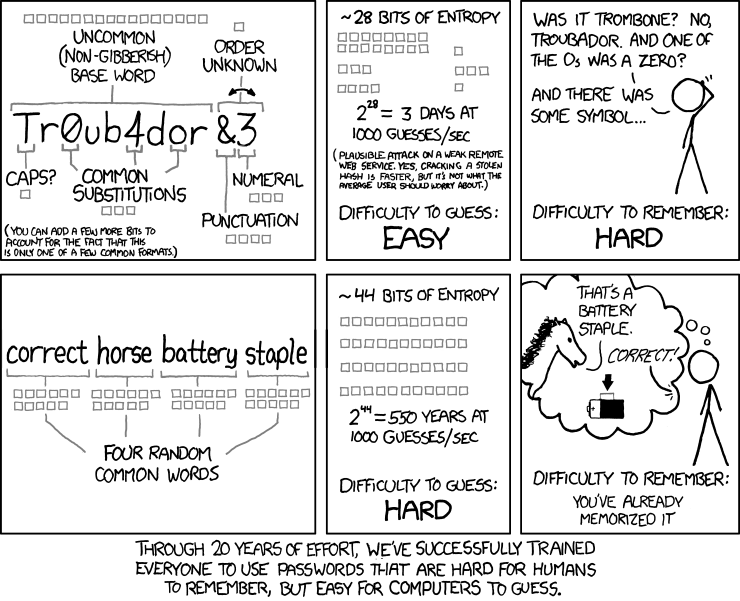
\includegraphics[width=\textwidth]{password_strength.png}

\newpage
\small
\setlength{\parindent}{0em}
\setlength{\parskip}{0.5em}

\subsubsection*{What is a Diceware passphrase?}

A passphrase is a bunch of words and characters that you type in to your computer to let it know for sure that the person typing is you. Passphrases differ from passwords only in length.

Diceware is a method for picking passphrases that uses dice to select words at random from a special list. Each word in the list is preceded by a four digit number. All the digits are between one and six, allowing you to use the outcomes of four dice rolls to select a word from the list.

\subsubsection*{Directions}

\begin{itemize}[leftmargin=*]

\item[1] Decide how many words you want in your passphrase. A four-word passphrase provides a level of security \textit{much} higher than the passwords most people use. For NSA-proof security, use seven.

\item[2] Roll all four dice at once and write the results down, reading from left to right, on a scrap paper. Make as many of these four-digit groups as you want words in your passphrase.

\item[3] Flip to the word list and look up the corresponding word next to each four-digit number.

\item[4] The words that you have found are your new passphrase! If required, capitalize a memorable word, and replace the last word with its four digit number.

\item[5] Come up with a way to remember your phrase. It might be a story, scenario, or sentence that that can remind you of the particular words you chose, in order.

\end{itemize}

\subsubsection*{Example}

Suppose you want a five-word passphrase. You will need $5 \times 4$ or 20 dice rolls. Let's say they come out as:

1, 6, 6, 6, 5, 1, 5, 6, 5, 3, 5, 6, 3, 2, 2, 3, 5, 6, 2, and 6. 

Write the results on a scrap of paper in groups of four:

1 6 6 6 \\
5 1 5 6 \\
5 3 5 6 \\
3 2 2 3 \\
5 6 2 6

You then look up each group of five rolls in the Diceware word list by finding the number in the list and writing down the word next to the number:

1666 cognitive \\
5156 poetic \\
5356 ribbon \\
3223 garlic \\
5626 smelliness

Your passphrase would then be:

cognitive poetic ribbon garlic smelliness

This passphrase is one of the 3,656,158,440,062,976 (about $2^{51}$) alternatives that could have been chosen by this method. 
